
%If our lexical priors -- our global conventions -- serve as a source of stability in meaning over longer timescales, then what accounts for our extraordinary flexibility  over short timescales? How do we coordinate on efficient local conventions, or \emph{conceptual pacts}, for talking about things we've never talked about before? In this section, we review the dynamics of coordination within repeated reference games and explore the possibility, formalized in Chapter 2, that rapid adaptation can be understood in a Bayesian modeling framework as lexical inference given partner-specific data.%: $P(\mathcal{L}_i | D_i, \Theta)$. 

When we first encounter a new communication partner in a new context, we call upon some representation about what we think different signals mean to them. 
In our account, this representation is given by $P(\Theta)$, the global background prior.
While we are agnostic to the exact function parameterized by $\Theta$, there are two properties that our account emphasizes.
First, this representation of meaning must be sensitive to the overall statistics of the population: there is more consensus about the meaning of \emph{dog} than the meaning of \emph{sclerotic aorta} in the general population. 
Second, this representation should also, in principle, be sensitive to the identity of the partner: a cardiologist should have different expectations about a new colleague than a new patient.

In this section, we 
The most well-known phenomenon in repeated reference games is a reduction in message length over multiple rounds \citeA{KraussWeinheimer64_ReferencePhrases, ClarkWilkesGibbs86_ReferringCollaborative}. 
The first time participants referred to a figure, they tend to use a lengthy, detailed description (``the upside-down martini glass in a wire stand'') but with a small number of repetitions -- between 3 to 6 times, depending on the pair -- the description is reduced down to the limit of just one or two words (``martini''). 
These final messages are as short or shorter than the messages participants choose for \emph{themselves} in the future  \citeA{FussellKrauss89_IntendedAudienceCommonGround} and are often incomprehensible to overhearers who were not present for the initial messages \cite{SchoberClark89_Overhearers}.
These observations set up the central empirical puzzle of convention formation: how does a short word or phrase that would have been completely ineffective for communicating under the initial lexical prior become perfectly understandable over mere minutes of interaction? What changes inside participants' minds in the interim? 

One simple non-social explanation --- that reduction is merely an effect of familiarity or repetition on the part of the speaker --- can be easily dispelled. 
When participants are asked to repeatedly refer to the same targets for a hypothetical partner, no reduction is found, and in some cases utterances actually get longer \cite{HupetChantraine92_CollaborationOrRepitition}. 
Whatever is changing must be a result of the \emph{interaction} between partners.
An alternative explanation suggested by our probabilistic model is that reduction is driven by \emph{ad hoc} word learning as communication partners coordinate on names. 
If long initial messages can be explained as the result of initial uncertainty in the lexical prior, as discussed in the previous section, then a decrease in uncertainty may license shorter messages.

There is some evidence supporting this alternative explanation in prior empirical work.
For example, \citeA{BrennanClark96_ConceptualPactsConversation} counted \emph{hedges} across repetitions.
Hedges are expressions like \emph{sort of} or \emph{like}, and morphemes like \emph{-ish}, that explicitly mark uncertainty or provisionality, such as \emph{a car, sort of silvery purple colored} \cite{BrennanClark96_ConceptualPactsConversation,Fraser10_Hedging,MedlockBriscoe07_HedgeClassification}.
If participants reduce their lexical uncertainty over successive rounds, then we might expect a corresponding decrease in explicit markers of this uncertainty. 
Indeed, \citeA{BrennanClark96_ConceptualPactsConversation} found a much greater occurrence of hedges on the first round than the final round (26\% and 2\%, respectively).
Additionally, very few hedges were found on early trials in less ambiguous contexts (e.g. referring to a shoe in the context of dogs and fish), lending support for the specific use of hedges to mark uncertainty rather than a generic social use when first beginning to talk with a new partner.

\subsection{Model simulations}

\begin{figure*}
\centering
    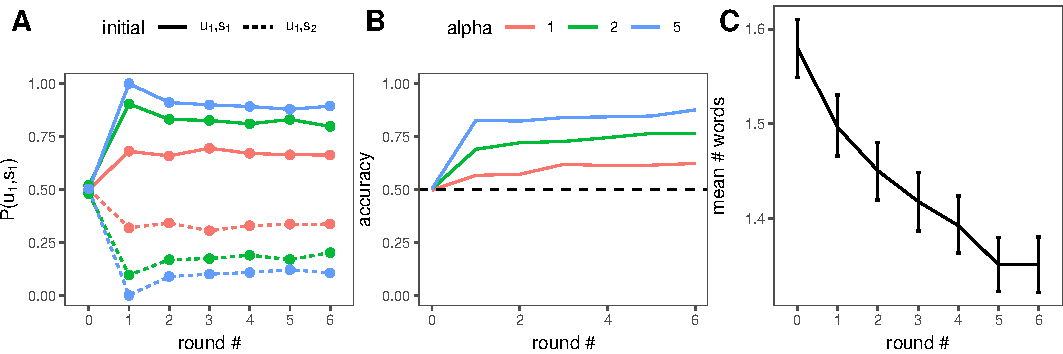
\includegraphics[scale=.8]{sec1-modelResults.pdf}
  \caption{Schematic of model}
  \label{fig:sec1model}
\end{figure*}


In this section, we show that the mechanism of uncertainty reduction is sufficient to produce reduction in utterance length across repeated interaction.

\paragraph{Simulation 1.1: Coordination}

First, we show how agents updating their meaning functions in this way can coordinate even in the absence of strong initial priors. 
The initial choices in an interaction can be taken as evidence for a particular lexicon and become the basis for successful communication, even when both speaker and listener are uncertain at the beginning.
As a simple test case, consider an environment with two objects ($\{o_1, o_2\}$), where the speaker must choose between two utterances ($\{u_1, u_2\}$) with equal production costs. 
For the prior $P(\mathcal{L})$ over the meaning of each utterance, we define a Beta distribution\footnote{In our implementation, we use exact enumeration over coarse-grained bins; experiments using variational inference on the full continuous distribution give similar results}, so on the first round both utterances are equally likely to apply to either shape. 
If the speaker were trying to get their partner to pick $o_1$, then because each utterance is equally (un)informative, they could only randomly sample one (say, $u_1$), and observe the listener's selection of a shape (say, $o_1$, a correct response). 
On the next round, the speaker uses the observed pair $\{u_1, o_1\}$ to update their beliefs about their partner's true lexicon, uses these beliefs to generate a new utterance, and so on. 
To examine expected dynamics over multiple rounds, we forward sample many possible trajectories.

We observe several important qualitative effects in our simulations. 
First, and more fundamentally, the evidence that a knowledgeable listener responded to utterance $u$ by choosing a particular object $o$ provides support for lexicons in which $u$ is a good fit for $o$. 
Hence, the likelihood of the speaker using $u$ to refer to $o$ will increase on subsequent rounds (see Fig.\ref{fig:sec1model}A). 
In other words, the initial symmetry between the meanings can be broken by initial random choices, leading to completely arbitrary but stable mappings in future rounds. 

Second, because the listener is updating their meaning representation from the same observations under the same set of assumptions, both partners converge on a \emph{shared} set of meanings; hence, the expected accuracy of selecting the target object rises on future rounds (see Fig. \ref{fig:sec1model}B). 
Third, because one's partner is assumed to be pragmatic via recursive Rational Speech Act mechanisms, agents can also learn about \emph{unheard} utterances. 
Observing $d = \{(u_1, o_1)\}$ also provides evidence that $u_2$ is \emph{not} a good fit for $o_1$.
This effect arises from Gricean maxims: if $u_2$ were a better fit for $o_1$, the speaker would have used it instead \cite{Grice75_LogicConversation}. 
Fourth, \emph{failed references} can lead to conventions just as effectively as successful references: if the speaker intends $o_1$ and says $u_1$, but then the listener incorrectly picks $o_2$, the speaker will take this as evidence that $u_1$ actually means $o_2$ in their partner's lexicon and become increasingly likely to use it that way on subsequent rounds.

\paragraph{Simulation 1.2: Reduction}

Next, we show how our model explains reduction of utterance length over multiple interactions. 
For utterances to be reduced, of course, they must vary in length, so we extend our grammar to include \emph{conjunctions}. 
Conjunctions are one of the simplest ways to constructi longer utterances compositionally from lexical primitives, using the product rule:
$$\mathcal{L}(u_i \textrm{ and } u_j, o) = \mathcal{L}(u_i, o) \times \mathcal{L}(u_j, o)$$
\indent Analogous to the \emph{tangram} stimuli used in the reference game reviewed in Chapter 1, which have many ambiguous features and figurative perspectives that may be evoked in speaker descriptions, we consider a scenario the two objects $\{o_1, o_2\}$ differ along two different features. 
The speaker thus has four primitive words at their disposal -- two words for the first feature ($\{u_{11}, u_{12}\}$) and two for the second $\{u_{21}, u_{22}\}$. 
While we established in the previous section that conventions can emerge over a reference game in the complete absence of initial preferences, players often bring such preferences to the table. 
A player who hears `ice skater' on the first round of a tangrams task is more likely to select some objects more than others, even though they still have some uncertainty over its meaning in the context. 
To show that our model can accommodate this fact, we allow the speaker's initial prior meanings to be slightly biased. 
We assume $u_{11}$ and $u_{21}$ are a priori more likely to mean $o_1$ and $u_{12}$ and $u_{22}$ are more likely to mean $o_2$.

We ran 1000 forward samples of 6 rounds of speaker-listener interaction, and averaged over the utterance length at each round \footnote{In our simulations, we used $\alpha = 10$ but found the basic reduction effect over a range of different biases}. 
Our results are shown in Figure \ref{fig:sec1model}C: the expected utterance length decreases systematically over each round. 
To illustrate in more detail how this dynamic is driven by an initial rational preference for redundancy relaxing as reference becomes more reliable, we walk step-by-step through a single trajectory. 
Consider a speaker who wants to refer to object $o_1$. 
They believe their knowledgeable partner is slightly more likely to interpret their language using a lexicon in which $u_{11}$ and $u_{12}$ apply to this object, due to their initial bias. 
However, there is still a reasonable chance that one or the other alone actually refers more strongly to $o_2$ in the true lexicon. 
Thus, it is useful to produce the conjunction "$u_{11}$ and $u_{12}$" to hedge against this possibility, despite its higher cost. 
Upon observing the listener's response (say, $o_1$), the evidence is indeterminate about the separate meanings of $u_{11}$ and $u_{12}$ but both become increasingly likely to refer to $o_1$. 
In the trade-off between informativity and cost, the shorter utterances remain probable options. 
Once the speaker chooses one of them, the symmetry collapses and that utterance remains most probable in future rounds. 
In this way, meaningful sub-phrases are omitted over time as the speaker becomes more confident about the true lexicon. 

\paragraph{Model comparison}
.
\todo[inline]{We should compare this model to several simpler baselines, e.g., no pragmatics, point estimate instead of uncertainty. It may also be useful to explicitly show that the simple Roth-Erev RL updating from this literature doesn't reduce.}

\subsection{Discussion}

Our model contrasts in several ways with prior theories of adaptation in language use. 
First, we contrast the mechanisms in our model with the lower-level priming mechanisms proposed in the influential \emph{interactive alignment} account \cite{pickering2004toward, pickering2006alignment, garrod2009joint}.
We fully expect that these low-level priming effects are at play in repeated reference tasks --- they are inescapable in any memory-based retrieval process.
However, the gradual reduction of the speaker's utterance length is not obviously primed by any features of the listener's language use; indeed, it happens even when the listener is prevented from saying anything at all and only feedback about the listener's accuracy is provided. 
Explaining why speakers think they can get away with shorter descriptions given sparse evidence of understanding (e.g. a correct response or a simple gesture of confirmation) and resort to longer descriptions given evidence of misunderstanding (e.g. an incorrect response) requires a mechanism for semantic coordination in the absence of lower-level statistics.

Second, we consider agent-based models implementing simple update rules \cite{steels_self-organizing_1995,barr_establishing_2004,young_evolution_2015}.
These models all share some mechanism that makes utterances more likely to be produced after communicative successes and less likely after communicative failures.
It is not clear why agents using such rules would initially prefer to produce longer utterance without some notion of uncertainty, or how naively reinforcing initially long descriptions could lead to reduction without some mechanism for \emph{credit assignment} to the component words.
It is plausible that using more sophisticated reinforcement schemes -- for instance, neural network architectures incorporating compositionality and recurrence into production \cite<e.g>{lazaridou2018emergence} -- could predict patterns of reduction with the addition of a cost term, but such a scheme would be much closer to our meta-learning approach, implemented using gradient-based learning \cite{hawkins2019continual}.

Our simulations in this section are also consistent with recent analyses of exactly \emph{what} gets reduced \cite{hawkins2020characterizing}.
Is the speaker adopting a fragment shorthand by randomly and noisily dropping words, or are they simplifying or narrowing their descriptions to names by systematically omitting redundant details?
Closed-class parts of speech like determiners and prepositions \emph{are} much more likely to be dropped than open-class parts of speech like adjectives and nouns, and entire modifying clauses are more likely to be dropped together than expected by random corruption.
This accords with early hand-tagged analyses by \citeA{Carroll80_NamingHedges}, which found that in three-quarters of transcripts from \citeA{KraussWeinheimer64_ReferencePhrases} the short names that participants converged upon were prominent in some syntactic construction at the beginning, often as a head noun that was initially modified or qualified by other information. 
These more fine-grained analyses suggest that reduction is grounded in the prior lexical content of the interaction and the speaker's increasing confidence in how the listener will interpret an initially ambiguous label. 

